\section{Basic theory}

\subsection{Overview}
\begin{frame}{Background}
	\begin{itemize}[<+->]
		\item Overview of image segmentation.
		\item Traditional: Accurate segmentation by Active Contour Model.
		\item Innovation: Deep learning methods.
	\end{itemize}
\end{frame}

\subsection{Mathematical Derivation}
\begin{frame}{Active Contour Model}
	\begin{block}{Curve evolution}
		We define curve as
		\begin{equation}
			\mathrm{C}(\theta,t)=(x(\theta,t),y(\theta,t))
		\end{equation}
		Then we have curvature
		\begin{equation}
			\frac{\partial \mathrm{C}(\theta,t)}{\partial t}=\mathrm{F}(k)N
		\end{equation}
		As constant evolution
		\begin{equation}
			\frac{\partial \mathrm{C}(\theta,t)}{\partial t}=V_0 N
		\end{equation}
		As curvature evolution
		\begin{equation}
			\frac{\partial \mathrm{C}(\theta,t)}{\partial t}=\alpha k N
		\end{equation}
	\end{block}
\end{frame}

\begin{frame}{Active Contour Model}
	\begin{block}{Level-set method}
		In curve $\mathrm{C}=\{(x,y),\phi(x,y)=c\}$ where $\phi(x,y)$ defined as level-set function, we introduce time $t$ and apply partial derivatives
		\begin{equation}
			\frac{\mathrm{d} \phi}{\mathrm{d} t}=\frac{\partial \phi}{\partial t}+\frac{\partial \phi}{\partial x}\cdot\frac{\partial x}{\partial t}+\frac{\partial \phi}{\partial y}\cdot\frac{\partial y}{\partial t}=\frac{\partial \phi}{\partial t}+\nabla\phi\cdot\frac{\partial (x,y)}{\partial t}=0
		\end{equation}
		$\nabla\phi=(\frac{\partial \phi}{\partial x},\frac{\partial \phi}{\partial y})$ is the gradient of level set function $\phi(x,y)$, and $\frac{\partial (x,y)}{\partial t}=\frac{\partial \mathrm{C}}{\partial t}=(\frac{\partial x}{\partial t},\frac{\partial y}{\partial t})=\vec{V}$. Then
		\begin{equation}
			\frac{\partial \phi}{\partial t}=-\nabla \phi \cdot \vec{V}=-|\nabla \phi| \cdot \frac{\vec{V}}{\nabla \phi}=|\nabla \phi| \cdot\left(-\frac{\nabla \phi}{|\nabla \phi|}\right) \cdot \vec{V}=|\nabla \phi| \cdot \vec{U} \cdot \vec{V}
		\end{equation}
	\end{block}
\end{frame}

\begin{frame}{Active Contour Model}
	\begin{block}{Calculus of variations}
		The 1D energy function can be written as
		\begin{equation}
			\mathrm{E}(\phi)=\int_{x_0}^{x_1}\mathrm{F}(x,\phi,\phi^\prime)\mathrm{d}x
		\end{equation}
		In order to apply Taylor's Formula, we introduce a very small $v(x)$
		\begin{equation}
			\mathrm{F}(x,\phi+v,\phi^\prime+v^\prime)=\mathrm{F}(x,\phi,\phi^\prime)+\frac{\partial \mathrm{F}}{\partial \phi}\cdot v+\frac{\partial \mathrm{F}}{\partial \phi^\prime}\cdot v+\cdots
		\end{equation}
		Intergrate both sides and collate to get
		\begin{equation}
			\mathrm{E}(\phi+v)-\mathrm{E}(\phi)=\int_{x_0}^{x_1}\left(v \frac{\partial \mathrm{F}}{\partial \phi}+v^{\prime} \frac{\partial \mathrm{F}}{\partial \phi^{\prime}}\right) \mathrm{d} x
		\end{equation}
	\end{block}
\end{frame}

\begin{frame}{Active Contour Model}
	\begin{block}{Calculus of variations}
		As $\phi(x_0)+v(x_0)=a,\phi(x_1)+v(x_1)=b$,
		\begin{equation}
			\int_{x_0}^{x_1} v^{\prime} \frac{\partial \mathrm{F}}{\partial \phi^{\prime}} \mathrm{d} x=\int_{x_0}^{x_1} \frac{\partial \mathrm{F}}{\partial \phi} \mathrm{d} v=\left.v \frac{\partial \mathrm{F}}{\partial \phi^{\prime}}\right|_{x_0} ^{x_1}-\int_{x_0}^{x_1} v \frac{\mathrm{d}}{\mathrm{d} x} \frac{\partial \mathrm{F}}{\partial \phi^{\prime}} \mathrm{d} x=-\int_{x_0}^{x_1} v \frac{\mathrm{d}}{\mathrm{d} x} \frac{\partial \mathrm{F}}{\partial \phi^{\prime}} \mathrm{d} x
		\end{equation}
		Ignoring very small changes in the independent variable, we have
		\begin{equation}
			\frac{\partial \mathrm{F}}{\partial \phi}-\frac{\mathrm{d}}{\mathrm{d}x}(\frac{\partial \mathrm{F}}{\partial \phi^\prime})=0
			\label{eq:1d}
		\end{equation}
		This is the Euler equation for 1D energy functional. Similarly, The Euler equation for 2D is
		\begin{equation}
			\frac{\partial \mathrm{F}}{\partial \phi}-\frac{\partial \mathrm{F}}{\partial \phi_x}-\frac{\partial \mathrm{F}}{\partial \phi_y}=0
		\end{equation}
	\end{block}
\end{frame}

\begin{frame}{Active Contour Model}
	\begin{block}{Calculus of variations}
		Take (\ref{eq:1d}) as an example. To solve the Euler equation, we introduce a small $v(\cdot)$
		\begin{equation}
			\mathrm{E}(\phi, t+\Delta t)=\mathrm{E}(\phi, t)+\Delta t \int_{x_0}^{x_1} \frac{\partial \phi}{\partial t}\left(\frac{\partial \mathrm{F}}{\partial \phi}-\frac{\mathrm{d}}{\mathrm{d} x}\left(\frac{\partial \mathrm{F}}{\partial \phi^{\prime}}\right)\right) \mathrm{d} x
		\end{equation}
		Let
		\begin{equation}
			\frac{\partial \phi}{\partial t}=-\left(\frac{\partial \mathrm{F}}{\partial \phi}-\frac{\mathrm{d}}{\mathrm{d} x}\left(\frac{\partial \mathrm{F}}{\partial \phi^{\prime}}\right)\right)=\frac{\mathrm{d}}{\mathrm{d} x}\left(\frac{\partial \mathrm{F}}{\partial \phi^{\prime}}\right)-\frac{\partial \mathrm{F}}{\partial \phi}
		\end{equation}
		Then
		\begin{equation}
			\Delta \mathrm{E}=\mathrm{E}(\phi,t+\Delta t)-\mathrm{E}(\phi,t)=-\Delta t\int\left(\frac{\partial \mathrm{F}}{\partial \phi}-\frac{\mathrm{d}}{\mathrm{d} x}\left(\frac{\partial \mathrm{F}}{\partial \phi^{\prime}}\right)\right)^2\mathrm{d}x
		\end{equation}
		The solution to the Euler equation of an energy functional tends to stabilize as the curve evolves, corresponding to the gradient flow of the given variation.
	\end{block}
\end{frame}

\begin{frame}{Active Contour Model}
	\begin{block}{Chan Vese Model}
		Chan and Vese proposed the Chan-Vese active contour model. Given a grayscale image $I(x)$, the target $\Omega_1$ and background $\Omega_2$ are detected with characteristic uniformity and a clear difference, represented by the approximate grayscale constants $c_1$ and $c_2$. The energy functional is defined as
		\begin{equation}
			\begin{aligned}
				\mathrm{F}\left(c_1, c_2, \phi\right) & =\lambda_1 \cdot \int_{\Omega}\left(\mathrm{I}(x)-c_1\right)^2 \cdot \mathrm{H}(\phi(x)) \mathrm{d} x+\lambda_2 \cdot \int_{\Omega}\left(\mathrm{I}(x)-c_2\right)^2 \cdot(1-\mathrm{H}(\phi(x))) \mathrm{d} x \\
				& +\mu \cdot \int_{\Omega} \delta_0(\phi(x))|\nabla \phi(x)| \mathrm{d} x+v \cdot \int_{\Omega} \mathrm{H}(\phi(x)) \mathrm{d} x
			\end{aligned}
		\end{equation}
		Where $\lambda_1,\lambda_2>0,\mu,v\geq0$. $\mathrm{H}(\phi)$ is the unit step function(Heaviside function). $\delta_0$ is its derivative, from which the Dirac function can be derived.
		\begin{equation}
			\mathrm{H}(z)=\left\{\begin{array}{ll}
				0 & z<0 \\
				1 & z \geq 0
			\end{array}, \delta_0(z)=\frac{\mathrm{d}}{\mathrm{d} z} \mathrm{H}(z)\right.
		\end{equation}
	\end{block}
\end{frame}

\begin{frame}{Active Contour Model}
	\begin{block}{Chan Vese Model}
		Substituting it into the Euler-Lagrange equation, the level set gradient flow of the Chan-Vese model is solved.
		\begin{equation}
			\frac{\partial \phi}{\partial \mathrm{t}}=-\frac{\partial \mathrm{F}}{\partial \phi}=\delta_{\varepsilon}\left\lfloor\mu \operatorname{div}\left(\frac{\nabla \phi}{|\nabla \phi|}\right)-v-\lambda_1\left(\mathrm{I}(x)-c_1\right)^2+\lambda_2\left(\mathrm{I}(x)-c_2\right)^2\right\rfloor
		\end{equation}
		where
		\begin{equation}
			c_1=\frac{\int \mathrm{I}(x) \cdot H(\phi(x)) \mathrm{d} x}{\int \mathrm{H}(\phi(x)) \mathrm{d} x}, \quad c_2=\frac{\int \mathrm{I}(x) \cdot(1-\mathrm{H}(\phi(x))) \mathrm{d} x}{\int(1-\mathrm{H}(\phi(x))) \mathrm{d} x}
		\end{equation}
	\end{block}
\end{frame}

\subsection{Dive into Deep Learning}
\begin{frame}{Neural Network}
	\begin{block}{Convolutional Neural Networks}
		\begin{itemize}
			\item convolutional layer
			\item pooling layer
			\item flatten layer
			\item fully connected layer
			\item activation layer
		\end{itemize}
	\end{block}
\end{frame}

\begin{frame}{Neural Network}
	\begin{figure}[h]
		\centering
		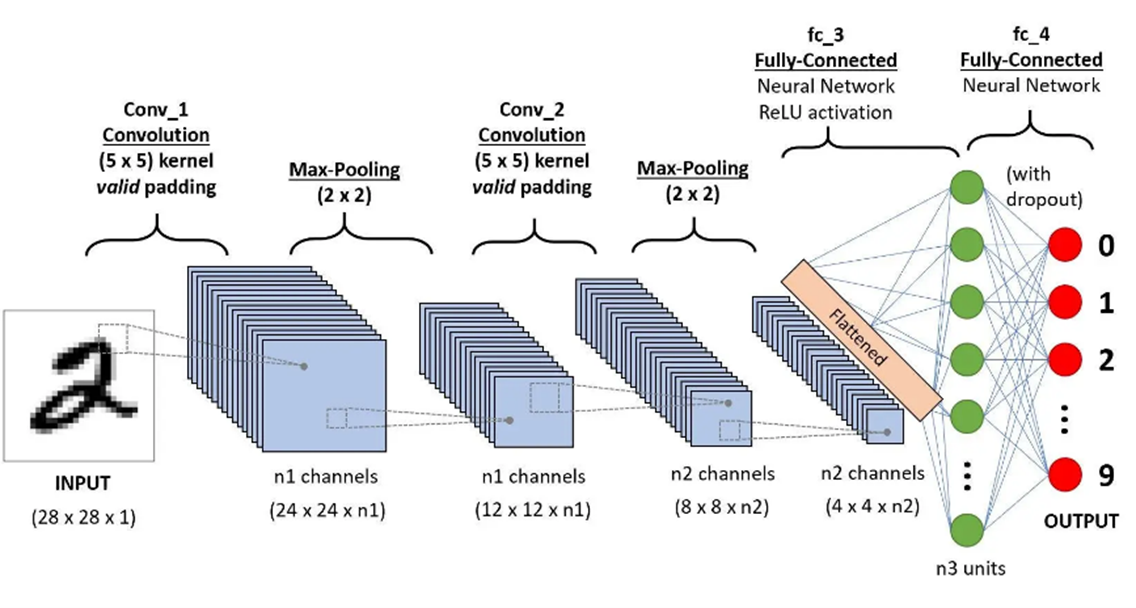
\includegraphics[width=0.8\textwidth]{images/num_rec.png}
		\caption{Handwritten number recognition pipeline}
		\label{fig:num_rec}
	\end{figure}
\end{frame}

\begin{frame}{Loss Functions}
	\begin{columns}
		\begin{column}{0.25\textwidth}
			\begin{block}{Softmax}
				\begin{equation}
					\text{Softmax}(x)=\frac{e^{x_i}}{\sum_i e^{x_i}}
				\end{equation}
			\end{block}
		\end{column}
		\pause
		\begin{column}{0.25\textwidth}
			\begin{block}{Sigmoid}
				\begin{equation}
					\text{Sigmoid}(x)=\frac{1}{1+e^{-x}}
				\end{equation}
			\end{block}
		\end{column}
		\pause
		\begin{column}{0.25\textwidth}
			\begin{block}{tanh}
				\begin{equation}
					\text{tanh}(x)=\frac{e^x-e^{-x}}{e^x+e^{-x}}
				\end{equation}
			\end{block}
		\end{column}
		\pause
		\begin{column}{0.25\textwidth}
			\begin{block}{ReLU}
				\begin{equation}
					\text{ReLU}(x)=\max(0,x)
				\end{equation}
			\end{block}
		\end{column}
	\end{columns}
\end{frame}

\begin{frame}{Optimizations}
	\begin{block}{Methods}
		\begin{itemize}
			\item Batch normalization
			\begin{equation}
				{\hat{x}}_i=\frac{x_i-\mu_B}{\sqrt{\sigma^2_B+\varepsilon}}
			\end{equation}
			\item Stochastic gradient descent
			\begin{equation}
				\theta=\theta-\eta\cdot\nabla_\theta J(\theta,x^{(i)},y^{(i)})
			\end{equation}
		\end{itemize}
	\end{block}
\end{frame}

\begin{frame}{Classic Models}
	\begin{columns}
		\begin{column}{0.5\textwidth}
			\begin{figure}[h]
				\centering
				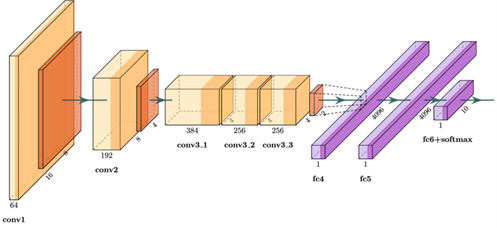
\includegraphics[width=0.75\columnwidth]{images/alexnet.png}
				\caption{AlexNet}
				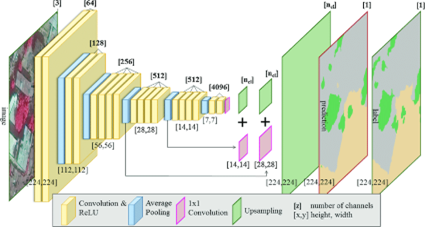
\includegraphics[width=0.7\columnwidth]{images/fcn.png}
				\caption{FCN}
			\end{figure}
		\end{column}
		\begin{column}{0.5\textwidth}
			\begin{figure}[h]
				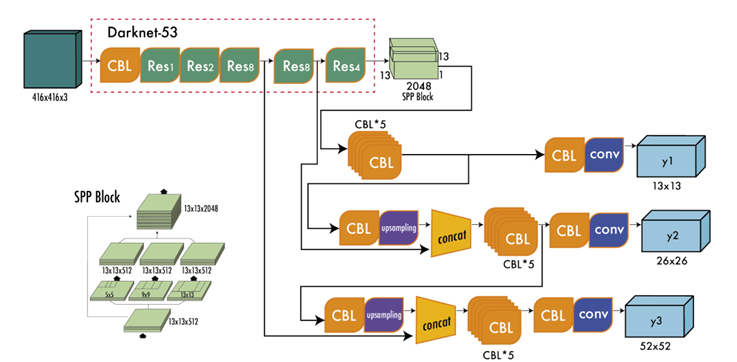
\includegraphics[width=0.7\columnwidth]{images/darknet.png}
				\caption{DarkNet}
				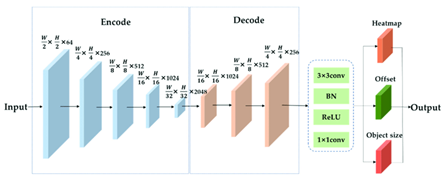
\includegraphics[width=0.75\columnwidth]{images/centernet.png}
				\caption{CenterNet}
			\end{figure}
		\end{column}
	\end{columns}
\end{frame}





